\documentclass[letterpaper,12pt]{exam}

\usepackage{ge05}
\usepackage{comment}
\usepackage{booktabs}
\usepackage{hyperref}
\urlstyle{rm}   % change fonts for url's (from Chad Jones)
\hypersetup{
    colorlinks=true,        % kills boxes
    allcolors=blue,
    pdfsubject={NYU Stern course GB 2303, Global Economy},
    pdfauthor={Dave Backus @ NYU},
    pdfstartview={FitH},
    pdfpagemode={UseNone},
%    pdfnewwindow=true,      % links in new window
%    linkcolor=blue,         % color of internal links
%    citecolor=blue,         % color of links to bibliography
%    filecolor=blue,         % color of file links
%    urlcolor=blue           % color of external links
% see:  http://www.tug.org/applications/hyperref/manual.html
}

\newcommand{\NX}{\mbox{\em NX\/}}
\newcommand{\POP}{\mbox{\em POP\/}}

\def\ClassName{The Global Economy}
\def\Category{Backus \& Cooley}
\def\HeadName{Practice Midterm Examination 1}

%\printanswers

\begin{document}
\parindent = 0.0in
\parskip = \bigskipamount
\thispagestyle{empty}%
\Head

\centerline{\large \bf \HeadName}%
%\centerline{March 9, 2005}
\centerline{Revised:  \today}

\bigskip
You have 90 minutes to complete this exam.  Please answer each
question in the space provided. You may consult one page of notes
and a calculator, but devices capable of wireless transmission are
prohibited.

I understand that the honor code applies: I will not lie, cheat,
or steal to gain an academic advantage, or tolerate those who do.

\begin{flushright}
\rule{4in}{0.5pt} \\ (Name and Signature)
\end{flushright}

{\it Note:  These questions come from old exams,
so the topics and numbers may be out of date.
But be assured:  good analysis lasts forever.}  \\

\begin{figure}[h]
    \centering
    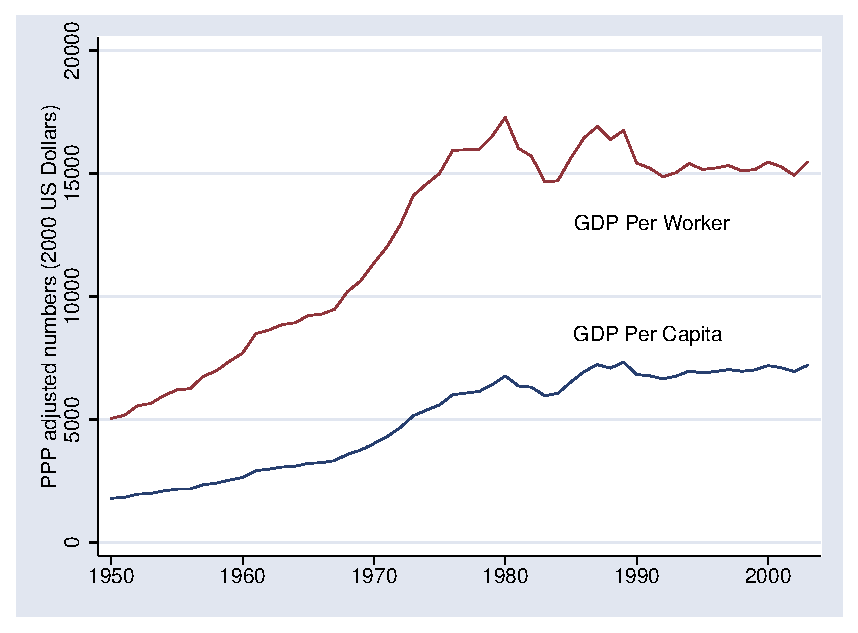
\includegraphics[scale=0.8]{pwtbramidterm07.eps}
    \caption{GDP Per Capita and GDP Per Worker in Brazil.}
    \label{fig:brazil}
\end{figure}

\begin{questions}
% ======================================================================
\question {\it Brazil.\/}
As a successful European investment banker, you
happen to have lunch with Rupert Murdoch.
Looking for a mutually beneficial topic of conversation,
you mention the limitless opportunities of Brazil,
which you've seen first-hand while arranging mergers
between Brazilian and European companies.
Murdoch calls your bluff, and asks why you see Brazil as an opportunity,
when its recent growth experience has been modest.
You change subjects after promising to send him a short
memo the next day.

Back in the office,
you ask your assistant to download some Brazilian data.
She collects the information in
Table \ref{tab:brazil} and Figure \ref{fig:brazil}.
In the table,
$\POP$ is population, $Y$ is real GDP, $L$ is employment
(the number of people working),
and $K$ is the stock of physical capital (plant and equipment).
Population is reported in millions;
the other numbers are PPP adjusted, reported in 2000 US dollars.
All come from the Penn World Tables, version 6.2.

Using this data, you do a few quick calculations.
Since the figure suggests a sharp change in 1980,
you decide to look separately at the periods before and after 1980.
%
\begin{parts}

\part You compute growth rates of GDP,
GDP per capita, and GDP per worker
for the two periods.
What are the important differences?
(15~points)

\part Since GDP per capita and GDP per worker are similar,
you decide to focus on the latter and
decompose its growth in each period into components
due to capital per worker and total factor productivity.
Which component accounts for the difference between
the two periods?
(15~points)

\part You are looking for a positive tone to your memo.
What exactly can you claim is growing in Brazil?  (10~points)

\end{parts}

\begin{table}
    \centering
    \tabcolsep = 0.2in
    \begin{tabular}{lcccc}
    \toprule
    Year     &  $ \POP $   &  $Y/\POP$   &  $Y/L$  &  $K/L$  \\
    \midrule
    1950 & \phantom{1}53,443  &   1,802  &  5,045   &  \phantom{1}8,559  \\
    1980 &   122,958  &   6,776  &  17,285\phantom{1}  & 39,064  \\
    2003 &   182,033  &   7,205  & 15,462\phantom{1} & 37,604    \\
    \bottomrule
    \end{tabular}
    \caption{Aggregate Data for Brazil.}
    \label{tab:brazil}
\end{table}


\begin{solution}
\begin{parts}
\part We compute continuously-compounded growth rates the usual way.
The results are summarized in below.
With both measures, growth effectively halted in 1980.
[Caveat:  this answer is only as good as the data that produced it.
There's been some controversy about whether this dataset
(``PPP adjusted'') measures real GDP appropriately.
There's no question growth rates have fallen, but the magnitude may be
overstated here.]

\begin{center}
    \begin{tabular}{lccccc}
    \toprule
    Period    &   $Y$ &  $Y/\POP$   &  $Y/L$  &  $K/L$  &  $A$ \\
    \midrule
    1950-1980 &  7.2 & 4.4 &  4.1  &  5.1   & 2.4  \\
    1980-2003 &  2.0 & 0.3 & (0.5) &  (0.2) & (0.4)  \\
    \bottomrule
    \end{tabular}
\end{center}

\part The usual growth accounting exercise.
First we compute TFP ($A$):
247 in 1950, 509 in 1980, and 462 in 2003.
Apparently TFP growth has disappeared.
The growth rates of the various components are listed above.
Our decomposition of the growth rate of output per worker is

\newpage
\[
        \gamma_{Y/L} \;=\; \gamma_A + \alpha \gamma_{K/L}
\]
with $\alpha = 1/3$.
For the two periods, we get
\begin{eqnarray*}
    \mbox{1950-1980:} &&  4.1  \;=\; 2.4 \mbox{ (A)} +  1.7 \mbox{ (K/L)}   \\
    \mbox{1980-2003:} &&  -0.5 \;=\; -0.4 \mbox{ (A)} -  0.1 \mbox{ (K/L)} .
\end{eqnarray*}

\part Anything sensible is fine.
Here's an attempt:
Although GDP per capita and GDP per worker are not growing,
GDP is, since there are more people, and more people working.
You have no way of knowing this, but there's also a difference
between the PPP-adjusted numbers reported in the Penn World Tables
and Brazil's official ``real GDP'' data.
Which you trust more is hard to say.
Despite all this, it's hard to avoid concern about the Brazilian
economy.
Going beyond what's in the exam,
I would add that Brazil now has a reasonably stable
political environment,
with several changes of government without major
changes in economic policy.
Long-term, that's a good thing, and could lead to
much better performance in the future.

\end{parts}
\end{solution}

%\pagebreak \phantom{xx} \pagebreak \phantom{xx} \pagebreak
% ======================================================================
\question {\it Vietnam.\/}
Since 1991, Vietnam's per capita GDP has
been growing at an average rate of 6.75\%, positioning the
Southeast Asian economy among the fastest growing in the world.
According to analysts, an obstacle to even speedier
growth will likely be removed shortly when Vietnam
joins the World Trade Organization.

Some facts.
In 2005, manufacturing and construction accounted for 41\% of GDP (up
from 38\% in 2001) and services for 38\% (from 27\%), whereas agriculture dropped to 21\% (from 23\%).
Employment is divided among the three sectors in the following
proportions: 17\%, 25\%, and 57\%, respectively (the service figure
includes 10\% in state employment). Female labor force participation
is high by world standards, with women accounting for 49\% of the
labor force. According to the World Bank, school enrollment rates
are 100\% in primary school, 70\% in secondary school, and 10\% in
university.

%\pagebreak % ****************
The most notable immediate effect of
WTO membership will be the scrapping of US quotas on garment imports
from Vietnam. While these quotas limit Vietnamese exports to the
US, some analysts warn that their removal may have a relatively
modest effect: the EU's decision to waive its import quotas this year
had only a small effect on shipments, probably because of strong
competition from other producers, particularly China.
A further difficulty is the spate of strikes in foreign-owned factories,
which led the government to raise the minimum wage paid by foreign firms
by 40\%.  See the attached article in {\it The Economist\/}.

\begin{parts}
\part
In which broad sectors is Vietnam likely to shift its
production in the next five years?  20 years?
Why? (10~points)

\part To comply with the conditions for WTO membership, the
Vietnamese National Assembly recently passed two pieces of
legislation that may have a substantial impact on the
economy. The Anti-corruption Law, which comes into effect June
1st, is intended to improve the detection and prevention of public
official corruption.  The Law on Investment, also
expected to come into effect in mid-2006, allows investment projects worth
less than \$1m to proceed without registration, and projects
valued at less than \$19m  will need to be registered but will not
require licenses.

Describe --- concretely --- how each of these changes are likely to effect
the economy's total factor productivity.
(10~points)

\part In your view, what government policies are likely to be
most effective in raising the living standard of the Vietnamese people
 over the next 25 years?  Why? (10~points)
\end{parts}

\begin{solution}
\begin{parts}
\part
In recent times, agriculture has fallen as a fraction of GDP,
and the other two sectors have increased their shares.
We'd expect that to continue for two reasons.
One is that this is a standard pattern for developing countries,
including the US 150 years ago:  people move off farms.
Another is that this reflects the (admittedly crude) productivities
implied by the GDP and employment shares:
17\% of the workforce produces 41\% of GDP in manufacturing
and construction,
whereas 57\% of the workforce produces only 21\% of GDP in agriculture.
Some of this might reflect differences in skill level
and capital per worker across industries, but it's likely that
productivity is lower in agriculture,
and that market forces will reallocate people from agriculture
into manufacturing --- and maybe services, too.

\part Each of these changes should reduce the cost of running a business,
which will increase TFP directly.
The investment law, in particular,
should make it easier to start new businesses,
which should facilitate the reallocation described above.
As the economy shifts resources to more productive sectors,
overall TFP will increase.
It's the same argument we used with international trade.


\part There are lots of sensible answers.
We'd stress flexible labor markets;
competitive product markets, including competition from abroad;
and a legal system that enforces property rights.

\end{parts}
\end{solution}

%\pagebreak %\phantom{xx} \pagebreak \phantom{xx} \pagebreak
% ======================================================================
\question {\it Miscellany.\/}
%
\begin{parts}
\part {\it Bridge to nowhere.\/}
In the context of our production function, would
the construction of an economically useless bridge in Alaska lead
(once it's completed)
to a change in total factor productivity?
Please explain your answer.  (10~points)

\part {\it Labor markets and trade.\/}
An analyst at the OECD commented that the difficulty Italy has had
adapting to increasing international trade
was a reflection of its rigid labor markets,
which discourage Italian businesses from the restructuring needed to
compete in global markets.
Do you find this argument persuasive?   Why or why not?  (10~points)

\part {\it Off-shoring.\/}
The term \textit{off-shoring} refers to
the relocation of work from one country (the US, say) to another
(India, for example).
Greg Mankiw, Bush's former economic advisor, suggested that
such trade in labor services was no different than
trade in goods:  the goal remains for countries
to perform those tasks it does relatively efficiently.
Do you agree?  Why or why not?
Would your answer change if you viewed the issue from the
perspective of the in-shoring country?  (10~points)
\end{parts}

\begin{solution}
\begin{parts}

\part TFP falls.  The production function is
\[
    Y \;=\; A K^\alpha L^{1-\alpha} .
\]
A new bridge increases the capital stock $K$.
If it leads to no additional output (it's ``useless'') then
$A$ must fall.

\part Sounds right to me.
Rigid labor markets make it difficult for
the Italian economy to shift people from
their current low-productivity jobs to
others.

\part Almost all economists, even liberal ones,
would agree with Mankiw:
have people do the jobs at which they are relatively most
productive.
In the long run, that produces a higher standard of living.
That's as true for one country as it is for the other.
Of course, individuals may be concerned with the disruption
that might generate in their own lives,
but there's little question where the greater good lies.
\end{parts}
\end{solution}

\end{questions}

%\pagebreak \phantom{xx} \pagebreak \phantom{xx}
%\end{document}
\newpage
Trouble at the mill \\
Jan 26th 2006 |  HANOI \\
From The Economist print edition

Strikes and pay rises afflict the new South-East Asian tiger

FACTORY workers in Vietnam have an extra reason to celebrate Tet, the lunar new year holiday that begins this weekend. Their government recently decided to raise the minimum wage in foreign-owned factories by up to 40\%, starting on February 1st. Pay packets in Hanoi and Ho Chi Minh City will now start at \$45 a month, the first mandated rise in several years. Experienced workers can expect an extra 7\% increase on top of that.

What is especially unsettling for investors is how the workers got their extra dough. Since late December, wildcat strikes have swept through the industrial zones surrounding Ho Chi Minh City. Tens of thousands of workers joined the protests over wages and conditions. Some of these turned violent, and machines were wrecked at one Taiwanese-owned plant. Bosses claim that outside agitators stoked the protests, distributing notes at factory gates while police stood idly by.

Apparently caught off-guard, the government issued a decree earlier this month raising the minimum wage in foreign-owned factories. Most strikers have now returned to work, but some have not, and investors are fuming over production stoppages and a higher wage bill. The European Chamber of Commerce has gone so far as to write a tart letter to the prime minister, Phan Van Khai, reminding him that investors set up shop in Vietnam precisely because ``the workforce is not prone to industrial action.''

At least, not until now. Workers in Vietnam have staged walkouts before, particularly over alleged mistreatment by foreign managers, but the scale and co-ordinated nature of the latest strikes are, well, striking. Some observers find it implausible that they could occur without the prior knowledge of the ruling party, which forbids independent trade unions. As in China, workers are allowed to join only a pliant, party-affiliated union.

Most of the affected factories are owned by East Asian companies, the biggest investors in Vietnam. At Song Than industrial zone, on the outskirts of Ho Chi Minh City, 80\% of the factories are owned by Taiwanese, producing clothing, shoes, furniture and bicycles for export. They grumble that higher wages will drive away foreign investment, running at \$5.8 billion last year, and give warning that Vietnam needs to stay competitive. ``Chinese wages are higher. But the quality and efficiency are also higher,� said Chen Chi Young, an official at Taiwan's de facto embassy.

So why didn't Vietnam crush the illegal strikes? One reason, say observers, may be internal jockeying ahead of the party congress in April, a five-yearly affair. The aim could have been to embarrass the provincial officials where the unrest began, or to burnish the leadership's credentials, or both. The factories most affected may also be a clue: Vietnam and Taiwan both claim ownership of the Spratly Islands, along with several other countries. On December 15th, Taiwan said it was building a landing strip on one of the islands.

Or perhaps the workers were simply fed up with low pay and stingy bosses, and were too numerous to repress. Vietnam has one of the world's fastest growing economies. Now it is learning that higher output means higher expectations.


%**********************************************************************
%**********************************************************************
\newpage
\def\HeadName{Practice Midterm Examination 2}
\parindent = 0.0in
\parskip = \bigskipamount
%\setcounter{page}{1}
\thispagestyle{empty}
\Head

\centerline{\large \bf \HeadName}%
\centerline{Revised:  \today}

\bigskip
You have 90 minutes to complete this exam.  Please answer each
question in the space provided. You may consult one page of notes
and a calculator, but devices capable of wireless transmission are
prohibited.

I understand that the honor code applies: I will not lie, cheat,
or steal to gain an academic advantage, or tolerate those who do.

\begin{flushright}
\rule{4in}{0.5pt} \\ (Name and Signature)
\end{flushright}

\begin{questions}
% ======================================================================
\question {\it Mexico and Turkey. }
Flextronics is an original equipment manufacturer of electronics,
making products around the world that are sold under
other brand names.
It is currently looking for a location  to produce
the next generation Xbox for Microsoft.
They would be sold (primarily) in the US and Europe.
Your mission:  to provide a quick assessment of the
productivity and labor market conditions for
two countries on the short list, Mexico and Turkey.
Mexico, of course, has both proximity to the US and access to the US
through NAFTA.
Turkey has proximity to Europe.

Recent data for the two countries includes
%
\begin{center}
%\tabcolsep = 0.12in
\begin{tabular}{lcccccc}
\toprule
        &  POP  &  Y/POP  &  L/POP  &  K/Y     &  Education &  Hours \\
\midrule
Mexico   & 104.3 &  7938 &  0.423 & 2.53  & 7.4  & 1871 \\%
Turkey   &  \phantom{1}71.3
                 &  5633 &  0.477 & 2.03  & 5.4  & 1918 \\%
\midrule
\end{tabular}
\end{center}
POP is population (millions), Y is GDP (2000 US dollars),
K is capital (2000 US dollars), Education is years of school,
and Hours is annual hours worked per employed person.
Y and K are PPP-adjusted.
Education and Hours are from the OECD's {\it Employment Outlook\/};
the other variables are from the Penn World Tables.

The World Bank's Doing Business website includes these measures
of labor market flexibility:
\begin{itemize}
\item Mexico:  difficulty of hiring workers (33),
rigidity of hours (40), difficulty of firing workers (70),
and cost of firing (52 weeks of salary).

\item Turkey:  difficulty of hiring workers (44),
rigidity of hours (40),  difficulty of firing workers (30),
and cost of firing (95 weeks of salary).
\end{itemize}
Low numbers indicate greater flexibility in each case.

\begin{parts}
\part Which country has higher total factor productivity?
(15~points)

\part Which country holds more risk of labor issues?
(15~points)

\part All things considered, which country do you think
is the better prospect?  Why?
(10~points)
\end{parts}

%\newpage
\begin{solution}
%
\begin{parts}
\part Calculations below.
%
\begin{center}
\begin{tabular}{lcccc}
\toprule
Country   &  $Y/\POP$  & $Y/L$   &  $K/L$ &  TFP ($A$)  \\
\midrule
Mexico        &  7.938  & 18.77  &  47.48 &  5.18 \\
Turkey        &  5.633  & 11.81  &  23.97 &  4.10 \\
Mexico/Turkey &  1.41   &  1.59  &  1.98  &  1.27 \\
\bottomrule
\end{tabular}
\end{center}
(NB:  I shifted the decimal point to make the numbers look
more reasonable.)

TFP is computed the simplest way:
from the production function
\begin{eqnarray*}
    Y/L  &=& A (K/L)^{1/3}
\end{eqnarray*}
If you look at the numbers, you see that Mexico has substantially
higher output per worker.
But that reflects, in part, a large disparity in
capital per worker (98\%).  Once that's taken into account,
we see that there's only a 27\% difference in total factor
productivity.
Since we'd expect Flextronics to bring the same amount
of capital to both locations, this is the relevant comparison.
There are, of course, many reasons why TFP might differ,
so it might be worth more thought.

\part Both countries have some labor market issues.
The biggest difference seems to reflect firing:
the indicators suggest that it's easier to fire workers
in Turkey, but more expensive.
Cost, quality, and flexibility of the labor market are
likely to be central issues to this decision.

\part This part is up to you.
\end{parts}
\end{solution}


%\pagebreak %\phantom{xx} \pagebreak %\phantom{xx} \pagebreak
% ======================================================================
\begin{table}[h!]
%    \tabcolsep = 0.2in
    \centering
    \begin{tabular}{lcccc}
    \toprule
    Indicator    &  China   &  India  &    UK   &  Source \\
    \midrule
    GDP per capita (USD) &  5,300  &  2,700 &  35,300  &  CIA Factbook \\
    GDP growth (\%)    &  11.2  &   8.4   &  2.9  &  The Economist \\
    Competitiveness  &  4.6    &  4.3   &  5.4  &  WEF \\
    Regulatory quality &  4.8 &  4.9  &  9.8  &  Governance Matters \\
    Rule of law   &  4.6  &  5.8  &  9.3  &  Governance Matters  \\
    Investor protection & 5  & 6  &  8  &  Doing Business \\
    Financial sophistication  &  3.3  &  4.9  &  6.2  &  WEF \\
    Macro stability    &  6.0  &  4.2  &  5.2  &  WEF  \\
    Control of corruption    & 3.8  &  5.3  &  9.4  & Governance Matters\\
    \bottomrule
    \end{tabular}
    \caption{Measures of performance and institutional quality
    in China, India, and the UK.
    Competitiveness index is an overall measure of institutional quality.}
    \label{tab:institutions}
\end{table}

\question {\it Investing in China and India.\/}
You work at a British asset management company and have been asked to
assess the potential of starting a country fund:
a mutual fund for UK investors
that would invest in China or India.
You realize that both countries are growing rapidly,
China more so to date than India,
but you wonder whether there are important
differences in the institutional environment
that might also be relevant.

Your summer intern collects the data in Table \ref{tab:institutions}
and explains what each of the indicators means.
In addition, she points out that
the World Economic Forum (WEF) collects survey responses about
the biggest problems faced by businesses.
In China they are:  access to financing, bureaucracy, corruption, and policy instability.
In India:  infrastructure, bureaucracy, labor regulations, and corruption. And in the UK:  taxes, education of workforce, and bureaucracy.

Based on this information and your own experience,
which country would you recommend? Why?
(30~points)


\begin{solution}
This is a relatively unstructured question,
there's no single best answer.
A good answer probably touches on the following points:
%
\begin{itemize}
\item Country performance.
The guess is that returns will reflect country performance.
To the extent China is growing faster,
it's probably the better bet.

\item General institutions.
Institutions are helpful for predicting future performance,
and for indicating whether that growth will be claimed
by the people who produce it.
If you look at ``competitiveness,'' the WEF's overall measure of
institutional quality, China ranks (slightly) higher.
Most measures will find little difference between them,
this one favors China by a small amount.
Corruption is an issue in both places, although there's
some indication that India controls it better.
Bureaucracy is an issue in both countries.
Political instability is mentioned as an issue in China,
and could be relevant in the sense that changing regulations
are difficult to deal with.

\pagebreak % ****
\item Investment-specific institutions.
There are specific institutions that pertain directly to financial
markets; as we've seen, it takes a lot of regulatory infrastructure
to make financial markets work well, even in developed countries.
Here India looks somewhat better than China.
Overall regulatory quality is better,
as are investor protection, rule of law, and financial sophistication. Access to financing is an issue in China,
but that's irrelevant to this endeavor.

\item Bottom line.  Your call.
It looks to me like India has, in some respects, more developed
institutions for capital market activity.
It's partly a matter of history, partly of how the countries
have evolved over the last 20 years.
It takes a fairly sophisticated set of institutions to get
bond and equity markets to work effectively,
and China probably has further to go in this dimension right now.
\end{itemize}

Grading:  30 points for an articulate
well-reasoned argument that hits these points
or otherwise makes a persuasive argument with the information
given in the question. Partial credit for other answers.
\end{solution}


%\pagebreak %\phantom{xx} \pagebreak %\phantom{xx} \pagebreak
% ======================================================================
\question {\it Miscellany.\/}
\begin{parts}

\part {\it Jobs.\/}
Senator Joe Lieberman once said something like:
``The only way to increase jobs is to make hiring attractive
to businesses.''
Use an analysis of the minimum wage to argue for or against
his statement.
(10~points)

\part {\it Infrastructure.\/}
An article posted on the discussion board suggested that infrastructure investments (highways, ports, telecommunications)
not only increase the stock of capital,
they  can also increase productivity.
Do you agree?  Why or why not?
(10~points)

\part {\it Trade balance.\/}
Some have suggested that the US trade deficit
($\NX < 0$) reflects inadequate saving,
while others have suggested that investment is excessive.
In what sense does each claim contain a grain of truth?
What evidence would you use  to support one claim over
the other?
(10~points)
\end{parts}

\begin{solution}
\begin{parts}
\part Sounds right to me.  The problem with the minimum wage
is that it makes hiring people less attractive to firms
(more expensive),
so they do less of it.

Grading:  10 points for clear elucidation of this point
and effective use of supply and demand diagram.

\part Infrastructure is clearly investment
(new capital goods), so it increases the stock of capital $K$,
which increases output $Y$.
It could also increase TFP through a number of routes:
perhaps a bottleneck makes particular investments worth
more than the production function suggests.
Or it allows more efficient production through some other means:
roads allow producers to sell to a larger market and exploit
economies of scale;
telecommunications might make use of efficient IT possible;
and so on.

Grading:  5 points for a clear argument that recognizes the
distinction between capital and productivity, 5 for a good
argument that infrastructure might raise productivity.

\part The grain of truth comes from the flow identity:
\[
    S \;=\; I + \NX.
\]
If $\NX <0$, that could come from low $S$ or high $I$.
If you look at this for the US, you see that $I$ has been
stable for 50 years, but $S$ has fallen over the last 25 years.
In that sense, it's the change in $S$ that is associated with
the change in $\NX$.

Grading:  7 points for noting the connection with the
identity, 3 for adding something to it that makes sense
for the US.

\end{parts}
\end{solution}

\end{questions}

%\pagebreak \phantom{xx} %\pagebreak \phantom{xx}

\vfill \centerline{\it \copyright \ \number\year \ NYU Stern
School of Business}

%**********************************************************************
%**********************************************************************
\newpage
\def\HeadName{Practice Midterm Examination 3}
\parindent = 0.0in
\parskip = \bigskipamount
%\setcounter{page}{1}
\thispagestyle{empty}
\Head

\centerline{\large \bf \HeadName}%
\centerline{Revised:  \today}

\bigskip
You have 90 minutes to complete this exam.  Please answer each
question in the space provided and show all of your work.
You may consult one page of notes and a calculator,
but devices capable of wireless transmission are prohibited.

I understand that the honor code applies: I will not lie, cheat,
or steal to gain an academic advantage, or tolerate those who do.

\begin{flushright}
\rule{4in}{0.5pt} \\ (Name and Signature)
\end{flushright}


\begin{questions}
% ======================================================================
\question {\it Indonesia.\/}
Indonesia is one of the world's most populous countries,
but it remains a poor one,
with GDP per capita of about 6 thousand US dollars.
Its recent trajectory, however, has been strong,
with average GDP growth over 5\% between 2000 and 2011
and a barely perceptible impact from the global financial crisis.

From EIU reports,
we find that Indonesia's recent success comes after a tumultuous history.
Following independence from the Dutch after World War II,
it had several decades of authoritarian rule.
The bloody transition from Sukarno to Suharto in 1965 is vividly portrayed in
Peter Weir's 1982 film, ``The Year of Living Dangerously.''
Economic performance improved under Suharto, but dissatisfaction
with authoritarian rule peaked after the Asian Crisis of 1997,
when the currency fell by 80\% against the dollar
and real GDP  fell 14\%.

After the crisis, Indonesia made a rapid transition to
multi-party democracy,
with the first democratic elections in 34 years in 1999
and several more since then.

Your mission is to examine the economic roots of recent success using
the data in Table \ref{tab:indonesia}.

\begin{parts}

\part What is the average annual growth rate of GDP per capita between
2000 and 2011?
GDP per worker?
(Here and elsewhere in this question,
growth rates are understood to be continuously-compounded.)
(10~points)

\part What was total factor productivity in 2000 and 2011?
Its average annual growth rate?
(10~points)

\part What are the other sources of growth?
What factors account for the growth rate of GDP per worker
you computed in (a)?
GDP per capita?
(10~points)
\end{parts}

\begin{table}
    \centering
    \tabcolsep = 0.2in
    \begin{tabular}{lrrrr}
    \toprule
    Year     &  $ \POP $   &  $Y/\POP$   &  $Y/L$  &  $K/L$  \\
    \midrule
    2000 &   220.0   &   4,151  & 8,828  & 21,408  \\
    2011 &   245.6   &   6,209  & 12,672 & 23,471  \\
    \bottomrule
    \end{tabular}
    \caption{Indonesia: aggregate data on output and inputs.
    Population is in millions.  The other numbers are 2005 US dollars
    (PPP adjusted, from Penn World Tables and EIU CountryData).}
    \label{tab:indonesia}
\end{table}


\begin{solution}
Short answers follow, see the accompanying spreadsheet for specific calculations.
\begin{parts}
\part The growth rate of GDP per capita is
\begin{eqnarray*}
    \gamma &=& \log (6.209/4.151)/(2011-2000) \;\;=\;\; 3.660\%.
\end{eqnarray*}
As always, $\log$ means the natural logarithm,
sometimes denoted {\tt LN}.
I moved the decimal point for convenience, but it has no affect on the growth rate.
Using the same method, the growth rate of GDP per worker is 3.286\%.

Grading:  5 points for correctly computing each number.

\part Productivity we find indirectly from
$ A = (Y/L)/(K/L)^\alpha$.
In 2000, we find
\begin{eqnarray*}
    A &=& (Y/L)/(K/L)^{1/3} \;\;=\;\; 8.828/21.408^{1/3}
    \;\;=\;\; 3.179 .
\end{eqnarray*}
If you don't move the decimal point, your numbers will be multiplied by 100.
In 2011, the same calculation gives us $A = 4.426$.
The growth rate is 3.007\%.

Grading:  4 points for each TFP number, 2 for its growth rate.

\part Growth in GDP per worker has these components:
\begin{eqnarray*}
    \gamma_{Y/L} &=&   \gamma_A  + \alpha \gamma_{K/L}  \\
    3.286     &=& 3.007  + 0.279 .
\end{eqnarray*}
Similarly, growth in GDP per capita is
\begin{eqnarray*}
    \gamma_{Y/POP} &=&  \gamma_{L/POP}  + \gamma_A
                + \alpha \gamma_{K/L}  \\
    3.660     &=& 0.374 + 3.007  + 0.279 .
\end{eqnarray*}
It's evident in both cases that productivity is the primary force
behind economic growth.
The bigger question, of course, is where the productivity came from.
That wasn't part, but it's not hard to imagine some improvement in institutions.
Some of that is evident in the next question.

Grading:  6 points for growth in GDP per worker and its components,
4 for the same with GDP per capita.
\end{parts}
\end{solution}


%\pagebreak \phantom{xx} \pagebreak \phantom{xx} \pagebreak
% ======================================================================
\question {\it Indonesia and Kazakhstan.\/}
As the junior member of a consulting team,
you have been asked to collect information on the pros and cons
of building a small manufacturing operation
in Indonesia or Kazakhstan.
The plant would produce toys aimed at the growing Asian market.
Both countries have shown recent signs of economic progress.
Both are actively recruiting foreign manufacturers,
Indonesia to continue its growth, Kazakhstan to diversify beyond its resource-based economy.

A collection of institutional indicators is given in Table \ref{tab:i-v-k}.
In addition, the political situations are quite different.
Indonesia is an emerging democracy.
The EIU describes Kazakhstan's political structure as authoritarian:
%
\begin{quote}
Nursultan Nazarbayev, the current president and formerly the first secretary of
the Communist Party of the Kazakh Soviet Socialist Republic, has ruled
Kazakhstan since independence.
He has steadily increased his control over Kazakhstan's political
structures, which has allowed him to secure re-election several times, the
most recent presidential election being in December 2005. Parliament
approved amendments that pave the way for
him to remain president for life.
His party, Nur Otan (Light-Fatherland),
won every seat available for
election in the new parliament.
\end{quote}
As a result, the political situation is thought to be stable.


\begin{table}[t]
\centering
\begin{tabular}{lrrrr}
\toprule
        &  \multicolumn{2}{c}{Indonesia} & \multicolumn{2}{c}{Kazakhstan}  \\
Indicator   &  1996   & 2010    & 1996  & 2010 \\
\midrule
\multicolumn{2}{l}{\it Governance} \\
Political stability (percentile)  &  13.5  &  18.9 & 28.4 & 61.8 \\
Govt effectiveness (percentile)   &  40.0  & 47.8  & 13.2 & 44.5 \\
Control of corruption (percentile) & 30.7  & 27.3  & 9.3  & 15.3 \\
\midrule
\multicolumn{2}{l}{\it Labor} \\
Minimum wage (ratio to average) & & 0.41 & & 0.13 \\
Severance after 10 years (weeks of pay) & & 56 & & 4 \\
Mandatory vacation (days per year)  && 0 & & 13 \\
Flexible hours?  (yes, no)  && yes & & yes \\
%Educational quality (percentile) && 69 && 25 \\
\midrule
\multicolumn{2}{l}{\it Transportation infrastructure} \\
Overall quality (percentile)  &&  42 && 40 \\
\midrule
\multicolumn{2}{l}{\it International trade} \\
Documents required (number) & & 4 & & 9 \\
Delay (days) &  & 17 & & 76 \\
Cost (USD per container) & & 644 & & 3130 \\
\bottomrule
\end{tabular}
\caption{Institutional indicators for Indonesia and Kazakhstan.}
\label{tab:i-v-k}
\end{table}


\begin{parts}
\part Which of these indicators are most important to your venture?
How do the two countries compare on them?
(10~points)
\part Which country or countries would you recommend to your clients?
What are the challenges they would face?
(10~points)
\end{parts}

\begin{solution}
\begin{parts}
\part All of these matter somewhat.  I'd say
labor is important in a manufacturing operation,
and also infrastructure and trade,
because you plan to export your product.
And political stability is important because
you want to know the climate won't quickly change for the worse.

Grading:  10 points for a clear logical argument that connects
the institutions to the demands of the business,
either this one or something else.
Partial credit for part thereof.

\part One thing you might do is rate the two countries along all
of these dimensions,
then come up with an overall grade based on your weighting of their importance.
A quick summary might be:
\begin{itemize}
\item Governance.  Both look ok.  The numbers aren't great,
but that's the challenge of operating in an emerging market.
(The benefit, of course, is low price.)
Curiously, Kazakhstan gets a better grade on political stability.
It's a bit worse, though, on corruption.

\item Labor.  Both countries have reasonably flexible
labor markets, although severance is higher in Indonesia.

\item Infrastructure and trade.
The big issue here is the delay in exporting (76 days!)
and cost of shipping a container --- both worse for Kazakhstan.
\end{itemize}
You could go either way, but I lean toward Indonesia,
which has become something
of a darling among emerging markets.

The World Economic Forum says:
``Indonesia remains one of the best-performing countries
within the developing Asia region.
Sound fiscal management has brought the budget deficit and
public debt down to very low levels, attributes that
contribute to further upgrading the country�s credit rating.
The situation is also improving,
albeit from a much lower base,
in the area of physical infrastructure.''
They also note that ``the quality of port facilities remains alarming''
and ``the electricity supply continues to be unreliable and scarce.''
As usual, some good, some bad.
They rate Indonesia 46th (of 142 countries), Kazakhstan 76th.
They're using information that goes beyond the question,
but I include it for background.

Grading:  10 points for a clear logical argument,
either this one or something else,
partial credit for part thereof.

\end{parts}
\end{solution}

%\pagebreak \phantom{xx} \pagebreak %\phantom{xx} \pagebreak
% ======================================================================
\question {\it True/false.\/}
Please explain why each statement is true, false, or uncertain.
The explanation is essential.
%
\begin{parts}
\part If a product is made in the Mexico but sold to consumers in the US,
it is not included in Mexican GDP.
(10~points)

\part If the unemployment rate falls, employment has risen.
(10~points)

\part Firms find it costly to search for workers with the right skills.
For that reason, regulations that discourage labor turnover are good for the economy.
(10~points)

\part A tax on labor tends to reduce employment.
(10~points)

\part In Ricardo's model, free trade is good for consumers but bad for workers.
(10~points)
\end{parts}

\begin{solution}
\begin{parts}
\part False.  GDP measures production in a country.  It doesn't matter who buys it.
\part Uncertain.  The issue here is that there are three categories:
employed, unemployed, and not in the labor force.
A lot of the action is in the last category.
So if some of the unemployed get jobs,
that lowers the unemployment rate and raises employment and the statement is true.
But if some of the unemployed leave the labor force,
we could see employment flat and the statement is false.
Or employment could fall, too, if the workers
leave the labor force without ever being unemployed.
In short, employment and unemployment can (and do) point in
different directions.


\part False.
Since the cost is borne by firms, they're in the best position
to act accordingly.
But reducing turnover by regulation will force firms to retain
workers even when that cost is outweighed by the benefits of a flexible workforce.

Think of the example of Spain where high severance and related requirements
discourages firms from hiring during expansions. This leads to a lower
level of employment on average.
It also leads to greater use of temporary workers who are
not subject to this requirement but must leave their jobs when their contracts expire.
In this case, raising the cost of firing workers actually increases turnover.

\part True.  Think of a supply/demand setup.
Consider a tax on labor paid by firms
(that's not essential, but it's helpful to be precise).
That will shift the demand curve down by the amount of the tax.
If demand slopes down and supply slopes up,
we'll see a decline in employment.
This isn't all that different from other products:
we tax cigarettes, for example, because we want to reduce the quantity.
This is the same logic.

\part False.
It's good for everyone.
More to the point:  workers and consumers are the same people,
both in Ricardo's model and the real world.

\end{parts}
%
Grading:  10 points for something like the answers above.
\end{solution}

\end{questions}

%\pagebreak \phantom{xx} %\pagebreak \phantom{xx}

\vfill \centerline{\it \copyright \ \number\year \ NYU Stern
School of Business}



\end{document}
